% Standalone TikZ figure: multi-partition hierarchical country -> within-country-cell
% classifier + offset regression (T3.4, CURRENT BEST MODEL, 182.9 +/- 7.0km full 5-fold CV,
% 2026-08-19). Supersedes figures/architecture.tex (T3.1, the single-partition version this
% one is built on top of -- kept as a historical record, not deleted, per this project's
% convention: see failed_experiments/ for the same principle applied to a failed attempt).
%
% Compile alone:      pdflatex architecture_t3_4.tex   (or lualatex/xelatex)
% Or embed in the writeup as a figure:
%   \begin{figure}[t]
%     \centering
%     \input{figures/architecture_t3_4_body}   % body-only include, see note at file end
%     \caption{Multi-partition hierarchical country/cell classifier + offset regression
%              (T3.4) -- current best model.}
%     \label{fig:architecture-t3-4}
%   \end{figure}
%
% All dimensions below are the real, verified numbers (src/protocol/param_check.py's
% check_compliance_multi_partition_model output, EfficientNet-B0 backbone, fold 0):
%   backbone feature dim = 1280, n_cells = 96 per partition (8/country x 12 countries),
%   K = 2 independent partitions, N_COUNTRIES = 12,
%   total params = 4,271,434 (of the 5,000,000 budget).
%
% What changed vs. T3.1 (figures/architecture.tex), and why -- see literature.md (CPlaNet)
% and Progress Tracker/Experiment_Design.md Tier 3 for the full reasoning:
%   - Backbone swapped MobileViT-XS (384px) -> EfficientNet-B0 (224px), same swap T3.1's own
%     3-backbone comparison already established as the winner -- not a T3.4-specific change.
%   - ONE cell partition (96 cells) -> TWO independent per-country partitions (96 cells each,
%     same MIN=40/MAX=120 density), built with different randomized KD-tree split-axis
%     choices on the SAME training points (src/protocol/geo_cells_multi.py).
%   - ONE cell head -> TWO parallel cell heads, each still hard-masked by country exactly as
%     in T3.1 (teacher-forced by true country at training, self-predicted at eval) -- the
%     masking mechanism itself is unchanged, just duplicated per partition.
%   - NEW: a blend step (spherical mean of the two predicted cells' centroids) between the
%     cell branches and the offset combine step -- this is the actual tested mechanism: two
%     independently-imperfect coarse decisions triangulate a finer point than either alone
%     (CPlaNet). Confirmed empirically: per-partition cell accuracy (~42%) was NOT better
%     than T3.1's single-partition accuracy (41.8%) -- the entire 10.1km/fold gain came from
%     this blend step, not from either head classifying better on its own.
%   - Offset head stays single/shared (not duplicated) -- it regresses relative to the
%     BLENDED centroid, not either partition's centroid individually.

\documentclass[tikz,border=4pt]{standalone}
\usetikzlibrary{positioning, arrows.meta, fit, backgrounds, shapes.geometric, calc}

\begin{document}
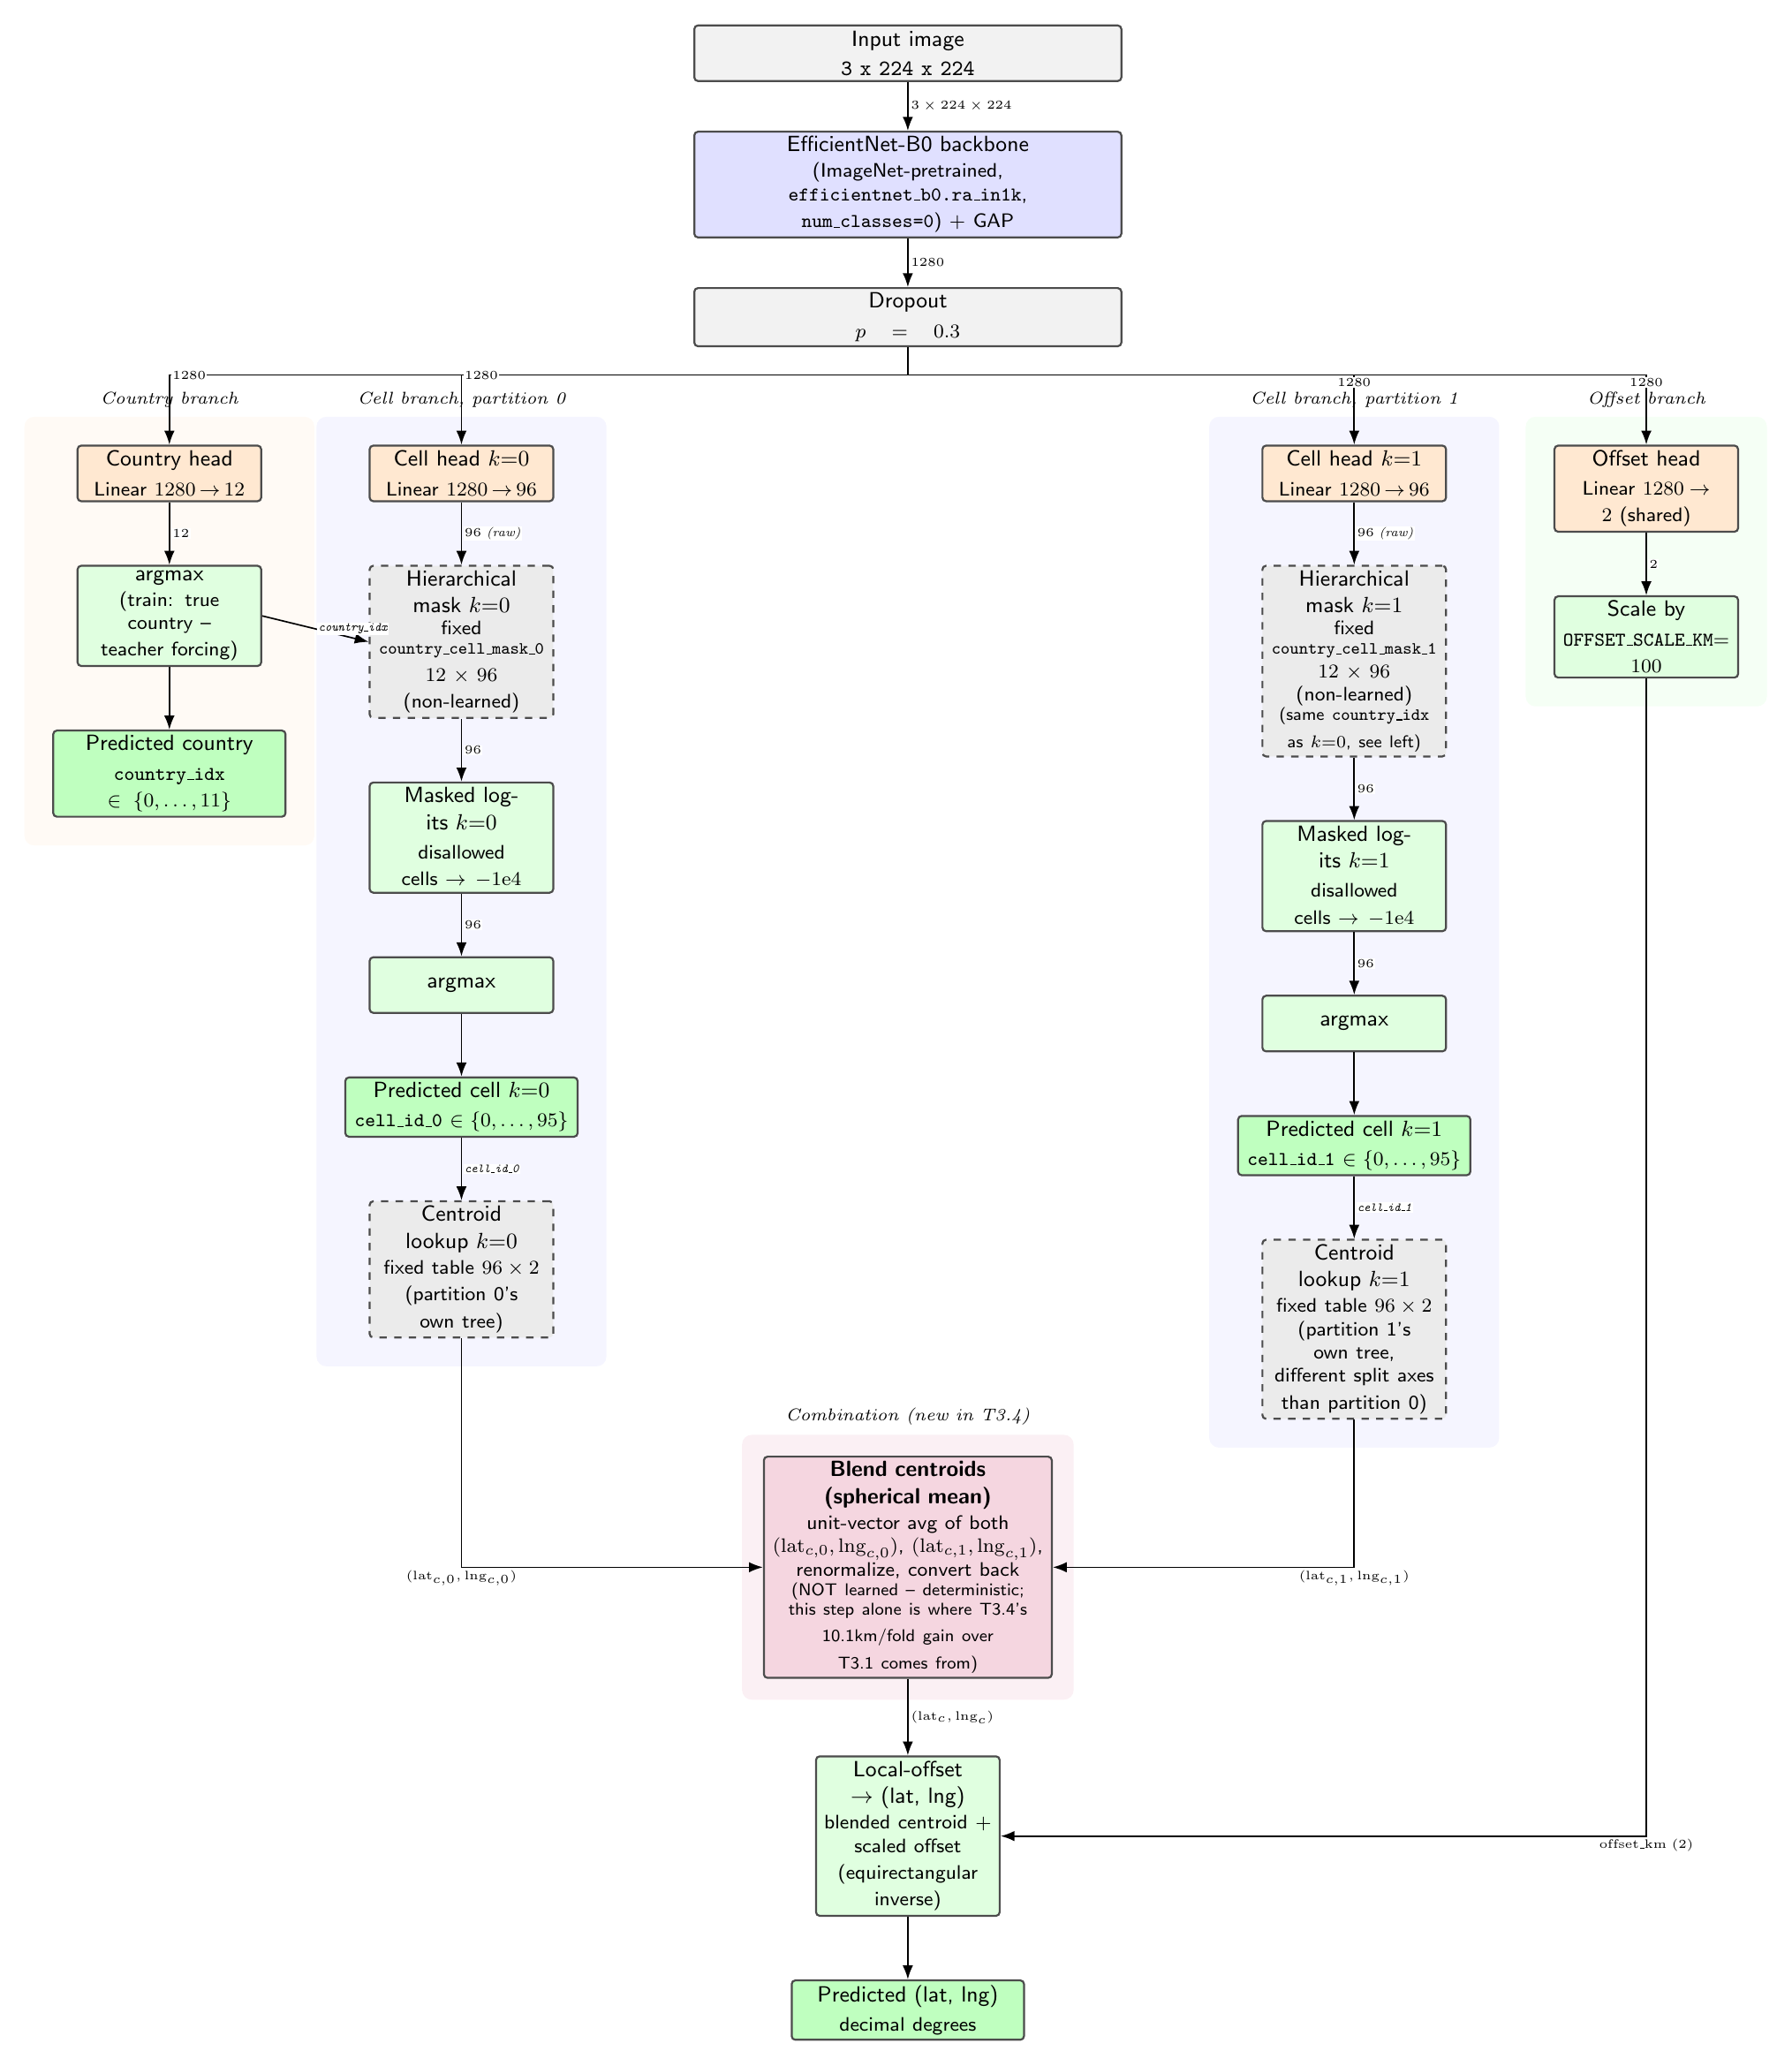
\begin{tikzpicture}[
  font=\sffamily\small,
  node distance=7mm and 10mm,
  >={Latex[length=2mm,width=1.5mm]},
  every path/.style={line width=0.6pt},
  block/.style={
    rectangle, rounded corners=1.5pt, draw=black!70, thick,
    minimum height=8mm, text width=28mm, align=center, inner sep=2pt
  },
  backbone/.style={block, fill=blue!12, text width=60mm},
  head/.style={block, fill=orange!18, text width=25mm},
  fixed/.style={block, fill=black!8, dashed, text width=25mm},
  op/.style={block, fill=green!12, text width=25mm},
  blend/.style={block, fill=purple!16, thick, text width=40mm},
  outnode/.style={block, fill=green!25, thick, text width=32mm},
  dimlabel/.style={font=\tiny\itshape, pos=0.5, right=0.5pt, fill=white, inner sep=0.5pt},
  dimlabelb/.style={font=\tiny\itshape, pos=0.5, below=0.5pt, fill=white, inner sep=0.5pt},
]

% ---- input / backbone / trunk (shared by ALL branches, incl. both partitions) ----
\node[block, fill=black!5, text width=60mm] (input) {Input image\\[1pt]\texttt{3 x 224 x 224}};
\node[backbone, below=of input] (backbone) {EfficientNet-B0 backbone\\[1pt]\footnotesize(ImageNet-pretrained, \texttt{efficientnet\_b0.ra\_in1k},\\ \texttt{num\_classes=0}) + GAP};
\node[block, fill=black!5, below=of backbone, text width=60mm] (dropout) {Dropout\\[1pt]\footnotesize $p=0.3$};

\draw[->] (input) -- (backbone) node[dimlabel]{$3\times224\times224$};
\draw[->] (backbone) -- (dropout) node[dimlabel]{$1280$};

% ---- four heads off the shared 1280-d feature: country, cell(partition 0), cell(partition 1), offset ----
\node[head, below left=14mm and 62mm of dropout] (country_head) {Country head\\[1pt]\footnotesize Linear $1280\!\to\!12$};
\node[head, below left=14mm and 20mm of dropout] (cell_head_0) {Cell head $k{=}0$\\[1pt]\footnotesize Linear $1280\!\to\!96$};
\node[head, below right=14mm and 20mm of dropout] (cell_head_1) {Cell head $k{=}1$\\[1pt]\footnotesize Linear $1280\!\to\!96$};
\node[head, below right=14mm and 62mm of dropout] (offset_head) {Offset head\\[1pt]\footnotesize Linear $1280\!\to\!2$ (shared)};

\draw[->] (dropout.south) -- ++(0,-4mm) -| (country_head.north) node[pos=0.2,dimlabel]{$1280$};
\draw[->] (dropout.south) -- ++(0,-4mm) -| (cell_head_0.north) node[pos=0.35,dimlabel]{$1280$};
\draw[->] (dropout.south) -- ++(0,-4mm) -| (cell_head_1.north) node[pos=0.65,dimlabelb]{$1280$};
\draw[->] (dropout.south) -- ++(0,-4mm) -| (offset_head.north) node[pos=0.8,dimlabelb]{$1280$};

% ---- country branch: argmax / teacher forcing ----
\node[op, below=9mm of country_head] (country_argmax) {argmax\\[1pt]\footnotesize (train: true country --\\ teacher forcing)};
\draw[->] (country_head) -- (country_argmax) node[dimlabel]{$12$};
\node[outnode, below=9mm of country_argmax] (country_out) {Predicted country\\[1pt]\footnotesize \texttt{country\_idx} $\in\{0,\dots,11\}$};
\draw[->] (country_argmax) -- (country_out);

% ---- cell branch, partition 0 (identical structure to T3.1's single cell branch) ----
\node[fixed, below=9mm of cell_head_0] (mask_0) {Hierarchical mask $k{=}0$\\[1pt]\footnotesize fixed \scriptsize\texttt{country\_cell\_mask\_0}\\\footnotesize $12\times96$ (non-learned)};
\draw[->] (cell_head_0) -- (mask_0) node[dimlabel]{$96$ (raw)};
\node[op, below=9mm of mask_0] (masked_0) {Masked logits $k{=}0$\\[1pt]\footnotesize disallowed cells $\to -1\mathrm{e}{4}$};
\draw[->] (mask_0) -- (masked_0) node[dimlabel]{$96$};
\node[op, below=9mm of masked_0] (argmax_0) {argmax};
\draw[->] (masked_0) -- (argmax_0) node[dimlabel]{$96$};
\node[outnode, below=9mm of argmax_0] (cellout_0) {Predicted cell $k{=}0$\\[1pt]\footnotesize \texttt{cell\_id\_0} $\in\{0,\dots,95\}$};
\draw[->] (argmax_0) -- (cellout_0);
\node[fixed, below=9mm of cellout_0] (centroid_0) {Centroid lookup $k{=}0$\\[1pt]\footnotesize fixed table $96\times2$\\ (partition 0's own tree)};
\draw[->] (cellout_0) -- (centroid_0) node[dimlabel]{\texttt{cell\_id\_0}};

% ---- cell branch, partition 1 (mirror of partition 0, independently randomized tree) ----
\node[fixed, below=9mm of cell_head_1] (mask_1) {Hierarchical mask $k{=}1$\\[1pt]\footnotesize fixed \scriptsize\texttt{country\_cell\_mask\_1}\\\footnotesize $12\times96$ (non-learned)\\ \scriptsize (same \texttt{country\_idx}\\ as $k{=}0$, see left)};
\draw[->] (cell_head_1) -- (mask_1) node[dimlabel]{$96$ (raw)};
\node[op, below=9mm of mask_1] (masked_1) {Masked logits $k{=}1$\\[1pt]\footnotesize disallowed cells $\to -1\mathrm{e}{4}$};
\draw[->] (mask_1) -- (masked_1) node[dimlabel]{$96$};
\node[op, below=9mm of masked_1] (argmax_1) {argmax};
\draw[->] (masked_1) -- (argmax_1) node[dimlabel]{$96$};
\node[outnode, below=9mm of argmax_1] (cellout_1) {Predicted cell $k{=}1$\\[1pt]\footnotesize \texttt{cell\_id\_1} $\in\{0,\dots,95\}$};
\draw[->] (argmax_1) -- (cellout_1);
\node[fixed, below=9mm of cellout_1] (centroid_1) {Centroid lookup $k{=}1$\\[1pt]\footnotesize fixed table $96\times2$\\ (partition 1's own tree,\\ different split axes\\ than partition 0)};
\draw[->] (cellout_1) -- (centroid_1) node[dimlabel]{\texttt{cell\_id\_1}};

% ---- country mask feeds BOTH partitions (same predicted country_idx, two masks) ----
% country_argmax and mask_0 sit in the same row, adjacent columns -- a direct horizontal
% line is unambiguous and crosses nothing. mask_1 (two columns further right, behind the
% whole partition-0 sub-tree) intentionally has NO drawn wire here -- routing one across the
% partition-0 column collided with its box text (caught on the first render); mask_1's own
% label notes "(same country_idx as k=0)" instead, which communicates the same fact without
% the crossing wire.
\draw[->] (country_argmax.east) -- (mask_0.west) node[pos=0.5, dimlabel]{\texttt{country\_idx}};

% ---- NEW vs. T3.1: blend the two partitions' predicted centroids (this is the tested mechanism) ----
\node[blend, below=11mm of $(centroid_0.south)!0.5!(centroid_1.south)$] (blend_node) {\textbf{Blend centroids (spherical mean)}\\[1pt]\footnotesize unit-vector avg of both\\ $(\mathrm{lat}_{c,0},\mathrm{lng}_{c,0})$, $(\mathrm{lat}_{c,1},\mathrm{lng}_{c,1})$,\\ renormalize, convert back\\ \scriptsize (NOT learned -- deterministic;\\ this step alone is where T3.4's\\ 10.1km/fold gain over T3.1 comes from)};
\draw[->] (centroid_0.south) |- (blend_node.west) node[pos=0.7, dimlabelb]{$(\mathrm{lat}_{c,0},\mathrm{lng}_{c,0})$};
\draw[->] (centroid_1.south) |- (blend_node.east) node[pos=0.7, dimlabelb]{$(\mathrm{lat}_{c,1},\mathrm{lng}_{c,1})$};

% ---- offset branch: scale ----
\node[op, below=9mm of offset_head] (offset_scale) {Scale by\\[1pt]\footnotesize \texttt{OFFSET\_SCALE\_KM}$=100$};
\draw[->] (offset_head) -- (offset_scale) node[dimlabel]{$2$};

% ---- combine blended centroid + offset ----
\node[op, below=11mm of blend_node] (combine) {Local-offset $\to$ (lat, lng)\\[1pt]\footnotesize blended centroid $+$\\ scaled offset\\ (equirectangular inverse)};
\draw[->] (blend_node) -- (combine) node[dimlabel]{$(\mathrm{lat}_c,\mathrm{lng}_c)$};
% Route straight down the offset column's own x (empty below offset_scale -- nothing else
% lives in that column) THEN across to combine at combine's own height, not the reverse --
% doing it the other way round cut a long horizontal line across the whole diagram at the
% wrong height on the first render (same class of bug as the country_idx wire above).
\draw[->] (offset_scale.south) -- ++(0,-6mm) |- (combine.east) node[pos=0.85, dimlabelb]{$\mathrm{offset\_km}\ (2)$};

\node[outnode, below=9mm of combine] (final) {Predicted (lat, lng)\\[1pt]\footnotesize decimal degrees};
\draw[->] (combine) -- (final);

% ---- background grouping boxes ----
\begin{scope}[on background layer]
  \node[fit=(country_head)(country_argmax)(country_out), fill=orange!4, rounded corners=4pt, inner sep=4mm, label={[font=\scriptsize\itshape]above:Country branch}] {};
  \node[fit=(cell_head_0)(mask_0)(masked_0)(argmax_0)(cellout_0)(centroid_0), fill=blue!4, rounded corners=4pt, inner sep=4mm, label={[font=\scriptsize\itshape]above:Cell branch, partition 0}] {};
  \node[fit=(cell_head_1)(mask_1)(masked_1)(argmax_1)(cellout_1)(centroid_1), fill=blue!4, rounded corners=4pt, inner sep=4mm, label={[font=\scriptsize\itshape]above:Cell branch, partition 1}] {};
  \node[fit=(offset_head)(offset_scale), fill=green!4, rounded corners=4pt, inner sep=4mm, label={[font=\scriptsize\itshape]above:Offset branch}] {};
  \node[fit=(blend_node), fill=purple!6, rounded corners=4pt, inner sep=3mm, label={[font=\scriptsize\itshape]above:Combination (new in T3.4)}] {};
\end{scope}

\end{tikzpicture}
\end{document}

% ---------------------------------------------------------------------------------------
% Params (verified via src/protocol/param_check.py's check_compliance_multi_partition_model):
%   backbone (EfficientNet-B0, efficientnet_b0.ra_in1k)  4,007,548
%   country head (1280->12)                                 15,372
%   cell head k=0 (1280->96)                                122,976
%   cell head k=1 (1280->96)                                122,976
%   offset head (1280->2, shared)                              2,562
%   total heads                                              263,886
%   TOTAL                                                  4,271,434   / 5,000,000 budget
%
% Full 5-fold CV result (2026-08-19, jobs 4055791-4055795, EfficientNet-B0, K=2 partitions,
% 224px, 100 epochs/fold): median km = 182.9 +/- 7.0 (beats T3.1's 193.0 +/- 4.2 on EVERY
% fold: -9.3, -4.8, -14.7, -10.7, -10.9km). cell acc (avg across partitions) = 42.1%,
% country acc = 72.7% -- both essentially unchanged from T3.1 (41.8%/72.8%), confirming the
% gain is from the blend step, not from either head classifying better individually.
% Current best model, gap to the ~114km reference target: 68.9km (down from T3.1's 79km).
% ---------------------------------------------------------------------------------------
